%%%%%%%%%%%%%%%%%%%%%%%%%%%%%%%%%%%%%%%%%%%%%%%%%%%%%%%%%%%%%%%%%%%%%%%%%%%%%%%%
%% Projeto Final de Graduação
%% Aluno: Victor Seixas Souza
%% Orientadora: Christiane Neme Campos
%% Tema: Teoria de Ramsey em Grafos
%%%%%%%%%%%%%%%%%%%%%%%%%%%%%%%%%%%%%%%%%%%%%%%%%%%%%%%%%%%%%%%%%%%%%%%%%%%%%%%%
% !TEX root = ../thesis.tex
%%%%%%%%%%%%%%%%%%%%%%%%%%%%%%%%%%%%%%%%%%%%%%%%%%%%%%%%%%%%%%%%%%%%%%%%%%%%%%%%

\chapter{Números de Ramsey para outros Grafos}
\label{chap:graph}

%%%%%%%%%%%%%%%%%%%%%%%%%%%%%%%%%%%%%%%%%%%%%%%%%%%%%%%%%%%%%%%%%%%%%%%%%%%%%%%%

Uma característica interessante da Teoria de Ramsey é sua possibilidade de diversas generalizações. Até agora, consideramos colorações que não tinham o grafo $K_r$ como subgrafo monocromático. Vamos relaxar esta condição e proibir outros grafos monocromáticos.

%%%%%%%%%%%%%%%%%%%%%%%%%%%%%%%%%%%%%%%%
\begin{definition}
Sejam $G$ e $H$ grafos simples. Definimos $r(G,H)$ como o menor inteiro positivo $n$, tal que qualquer coloração de arestas em duas cores do grafo $K_n$ possui um $G$ da primeira cor ou um $H$ da segunda cor.
\end{definition}
%%%%%%%%%%%%%%%%%%%%%%%%%%%%%%%%%%%%%%%%

Note que por esta definição, $R(k,s) = r(K_k, K_s)$. Também definimos $r(G) = r(G,G)$. Segue da definição que se $G$ é subgrafo de $G'$ então $r(G,H) \leq r(G',H)$. Assim, estes números estão bem definidos pois $r(G,H) \leq r(K_{v(G)}, K_{v(H)}) = R(v(G), v(H)) < \infty$. De maneira análoga, podemos definir os números de Ramsey para várias cores, $r(G_1, \dots, G_k)$, e adaptar a notação $r_k(G) = r(G,\dots,G)$.

Neste capítulo, vamos estudar algumas classes de grafos interessantes e seus números de Ramsey. Vale observar que mesmo para famílias simples de grafos, os números de Ramsey associados podem ser bem difíceis de se determinar. Por este motivo, muitos dos resultados apresentados nesta seção não incluirão as demonstrações. O texto, no entanto, fornece uma base sólida o suficiente para que o leitor interessado, busque as referências e estudem tais demonstrações por si só.

%%%%%%%%%%%%%%%%%%%%%%%%%%%%%%%%%%%%%%%%%%%%%%%%%%%%%%%%%%%%%%%%%%%%%%%%%%%%%%%%

\section{Grafos Bipartidos}

Seja $G = (V,E)$ um grafo simples. Dizemos que $G$ é um \indef{grafo bipartido} se o conjunto $V$ pode ser particionado em duas partes não vazias $X$ e $Y$ de tal forma que toda aresta em $E$ tem uma extremidade em $X$ e a outra em $Y$. Tal partição $\{ X,Y \}$ é dita uma \indef{bipartição} do grafo $G$. Um grafo $G$ com bipartição $\{X,Y\}$ é denotado $G[X,Y]$.

Quando um grafo bipartido $G[X,Y]$ é tal que todo par de vértices $x \in X$ e $y \in Y$ é adjacente, dizemos que $G[X,Y]$ é um \indef{grafo bipartido completo}. Naturalmente, temos uma família associada aos grafos com esta propriedade. Denotamos por $K_{m,n}$ o grafo bipartido completo $G[X,Y]$ com $|X| = m$ e $|Y| = n$. Por construção, note que $v(K_{m,n}) = m + n$ e $e(K_{m,n}) = mn$. A Figura~\ref{graph:fig:part} ilustra alguns exemplos de grafos bipartidos completos.

%%%%%%%%%%%%%%%%%%%%%%%%%%%%%%%%%%%%%%%%
\begin{figure}[ht!]
\centering
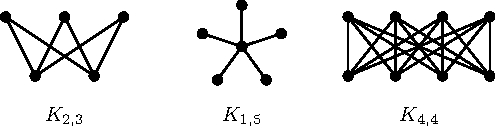
\includegraphics{figures/3_graph_1_part}
\caption{Alguns grafos bipartidos completos.}
\label{graph:fig:part}
\end{figure}
%%%%%%%%%%%%%%%%%%%%%%%%%%%%%%%%%%%%%%%%

Podemos generalizar o conceito de bipartição de um grafo. Se for possível particionar o conjunto de vértices em $k$ partes não vazias de maneira que toda aresta do grafo possui extremidades em partes distintas, dizemos que o grafo é $k$-\emph{partido}. Um grafo bipartido é, portanto, 2-partido. Denotamos por $K_{a_1, \dots, a_k}$ o grafo completo $k$-partido com $n$ partes, cuja $i$-ésima parte possui $a_i$ vértices. Quando $a_1 = a_2 = \dots = a_k$, obtemos grafos que fazem parte de uma família de grafos conhecida como \indef{grafos de Turán}\footnote{Os grafos de Turán são grafos completos $r$-partidos com as partes de tamanho mais próximas possíveis. Isto é, são grafos da forma $K_{a_1, \dots, a_r}$ com $|a_i - a_j| \leq 1$ para todo $1 \leq i,j \leq r$.}.
Denotamos os grafos de Turán que possuem todas as partes iguals por $T_r(k) = K_{k, \dots, k}$, ou seja, $T_r(k)$ é o grafo completo $r$-partido com partes de tamanho $k$ cada. Nas próximas seções, mostramos que estes grafos são bem interessantes para construir limitantes inferiores para números de Ramsey.

Um subcaso notável dos grafos bipartidos completos são os \indef{grafos estrela} $K_{1,n}$. O desenho do $K_{1,5}$,na Figura~\ref{graph:fig:part}, evidencia a motivação por trás deste nome. Podemos caracterizar os números de Ramsey $r(K_{1,n}, K_{1,m})$ da seguinte forma.

%%%%%%%%%%%%%%%%%%%%%%%%%%%%%%%%%%%%%%%%
\begin{theorem}[Harary~\cite{harary}]
Sejam $m$ e $n$ inteiros positivos, temos que
\[r(K_{1,m}, K_{1,n}) = \begin{cases}
  m + n , & \text{se } m \text{ ou } n  \text{ forem ímpares;} \\
  m + n - 1, & \text{se } m \text{ e } n \text{ forem pares.}
\end{cases}\]
\end{theorem}
%%%%%%%%%%%%%%%%%%%%%%%%%%%%%%%%%%%%%%%%
\begin{proof}
Primeiramente, note que em uma coloração de arestas, um $K_{1,m}$ monocromático na cor $C$ corresponde a um vértice $v$ tal que $d_C(v) \geq m$.

Considere uma $RB$-coloração qualquer de um grafo completo $G$ sem $K_{1,m}$ vermelho ou $K_{1,n}$ azul. Então $d_R(v) \leq m-1$ e $d_B(v) \leq n-1$ para todo vértice $v \in V(G)$. Isto é impossível se $G = K_{m+n}$, logo $r(K_{1,m}, K_{1,n}) \leq m+n$.
Se $m$ e $n$ são pares, considere $G = K_{m+n-1}$. Temos, portanto, que $d_R(v) = m-1$ e $d_B(v) = n-1$ para todo vértice $v \in V(G)$. Logo, o grafo $G_R$ possui todos os vértices de grau ímpar. Ademais, $v(G_R) = m + n -1$ também é ímpar. Pelo \emph{Handshaking Lemma}, não existe grafo com um número ímpar de vértices de grau ímpar. Portanto, $r(K_{1,m}, K_{1,n}) \leq m + n - 1$.

No caso de algum entre $m$ e $n$ ser ímpar, suponha, sem perda de generalidade, que $m$ seja ímpar, com $m = 2k + 1$. Considere $G  = K_{m+n-1}$ com $V(G) = \{ v_0, \dots, v_{m+n-2} \}$. Defina uma $RB$-coloração $c$ da seguinte maneira.
\[c(v_i v_j) = \begin{cases}
  \text{vermelho}, & \text{se }  |i - j| \equiv 1, 2, \dots, \text{ou } k \Mod{m+n-1}; \\
  \text{azul}, & \text{caso contrário}.
\end{cases}\]
Note que nesta coloração, $d_R(v) = 2k = m - 1$ e $d_B(v) = n - 1$, para todo vértice $v \in V(G)$. Portanto, $c$ não possui $K_{1,m}$ vermelho nem $K_{1,n}$ azul, o que implica em $r(K_{1,m}, K_{1,n}) = m + n$.

Suponha, agora, que ambos $m$ e $n$ sejam pares. Considere um grafo bipartido $G = G[X,Y]$, com $X = \{ x_i : i \in \Z{l} \}$ e $Y = \{ y_i : i \in \Z{l} \}$, tal que os vértices $x_i$ e $y_j$ são adjacentes se e somente se $i - j \equiv 1, 2, \dots, \text{ou } k \Mod{l}$. Note que $G$ é $k$-regular, e seu complemento é $(2l - k - 1)$-regular.
Escolhendo $l = \frac{m + n -2}{2}$ e $k = m-1$, temos que $G$ é um grafo com $m + n - 2$ vértices que é $(m-1)$-regular com complementar $\comp{G}$ $(n-2)$-regular. Isto corresponde a uma coloração de $K_{m + n - 2}$ sem $K_{1,m}$ vermelho nem $K_{1,n}$ azul. Portanto, temos $r(K_{1,m}, K_{1,n}) = m + n - 1$.
\end{proof}
%%%%%%%%%%%%%%%%%%%%%%%%%%%%%%%%%%%%%%%%

Este resultado pode ser generalizado com idéias parecidas para o número de Ramsey com diversas cores.

%%%%%%%%%%%%%%%%%%%%%%%%%%%%%%%%%%%%%%%%
\begin{noprooftheorem}[Burr, Roberts~\cite{burr1973ramsey}]
Sejam $m_1, \dots, m_k$ inteiros positivos, $t$ dos quais são pares. Temos que
\[r(K_{1,m_1}, \dotsc,  K_{1,m_k}) = \sum_{i=1}^{k} m_i  - k + \varepsilon,\]
onde $\varepsilon = 1$, se $t$ é par, e $\varepsilon = 2$, caso contrário.
\end{noprooftheorem}
%%%%%%%%%%%%%%%%%%%%%%%%%%%%%%%%%%%%%%%%

Outras classes de grafos bipartidos completos também já foram estudadas. Por exemplo, sabe-se que, para todo $n\geq 2$, $r(K_{2,n}, K_{2,n}) \leq 4n -2$~\cite{exoo}. Além disso, conjectura-se que $4n - 3 \leq r(K_{2,n}, K_{2,n}) \leq 4n -2$~\cite{lortz2002ramsey}.
O compêndio dinâmico de Radziszowski~\cite{small_ramsey} é uma excelente referência para encontrar outros resultados deste tipo.

%%%%%%%%%%%%%%%%%%%%%%%%%%%%%%%%%%%%%%%%%%%%%%%%%%%%%%%%%%%%%%%%%%%%%%%%%%%%%%%%

\section{Caminhos e Ciclos}

Um \indef{caminho} é um grafo simples que pode ter seus vértices arranjados em uma sequência linear, de modo que dois vértices são adjacentes, se e somente se, correspondem a elementos consecutivos na sequência. Similarmente, um \indef{ciclo} é um grafo simples com $n \geq 3$ que pode ter seus vértices arranjados em uma sequência linear cíclica, de modo que dois vértices são adjacentes, se e somente se, correspondem a elementos consecutivos na sequência.

%%%%%%%%%%%%%%%%%%%%%%%%%%%%%%%%%%%%%%%%
\begin{figure}[ht!]
\centering
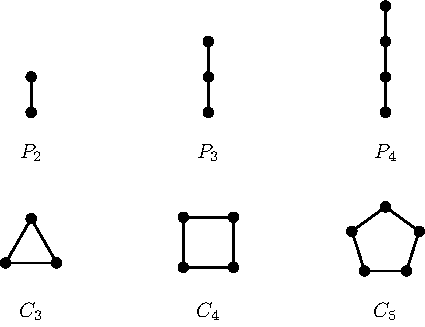
\includegraphics{figures/3_graph_2_cyclepath}
\caption{Alguns caminhos e ciclos pequenos.}
\label{graph:fig:cyclepath}
\end{figure}
%%%%%%%%%%%%%%%%%%%%%%%%%%%%%%%%%%%%%%%%

Caminhos e ciclos também são agrupadas em famílias de grafos. Os \indef{grafos caminhos} são grafos simples com $n$ vértices e $n-1$ arestas, isomorfos ao grafo $(\{v_1,\dots,v_n\}, \{v_iv_{i+1}: 1\leq i < n\})$. Já os \emph{grafos ciclos} são grafos com $n$ vértices, $n\geq 3$, e $n$ arestas isomorfos ao grafo $(\{v_1,\dots,v_n\}, \{v_iv_{i+1}: 1\leq i < n\} \cup v_1v_n)$. Ambas as famílias estão exemplificadas na Figura~\ref{graph:fig:cyclepath}.
Note que $P_2 \iso K_2$, $P_3 \iso K_{1,2}$, $C_3 \iso K_3$ e $C_4 \iso K_{2,2}$.

Note que se $n>1$, o grafo $P_n$ possui dois vértices de grau um, chamados de \indef{extremidades}; os demais $n-2$ vértices são ditos \indef{internos} e possuem grau dois. Já o grafo $C_n$ é 2-regular, isto é, todos os seus vértices possuem grau dois e pode ser visto como um grafo obtido pela adição de uma aresta ligando as extremidades de um $P_n$.

Caminhos e ciclos são de importância fundamental para a Teoria de Grafos, sendo peças centrais em muitas de suas subáreas. Naturalmente, números de Ramsey que envolvem estes grafos foram intensamente estudados. Uma primeira família de números de Ramsey envolvendo caminhos e ciclos está explicitada a seguir.

%%%%%%%%%%%%%%%%%%%%%%%%%%%%%%%%%%%%%%%%
\begin{proposition}
\label{graph:thm:rpt}  Para todo $k \geq 1$, temos
\[r(P_k, K_3) = r(P_k, C_3) = 2k - 1.\]
\end{proposition}
%%%%%%%%%%%%%%%%%%%%%%%%%%%%%%%%%%%%%%%%
\begin{proof}
Note que o grafo $K_{k-1,k-1}$ não possui triângulo e que o seu complementar é formado por duas cópias disjuntas de $K_{k-1}$, e assim, não possui $P_k$. Dessa forma, o grafo $K_{k-1,k-1}$ induz uma $RB$-coloração do $K_{2k - 2}$ sem $K_3$ azul e sem $P_k$ vermelho. Isto nos mostra que $r(P_k, K_3) > 2k - 2$.

Agora, considere uma $RB$-coloração $c$ de $G=K_n$, com $n = 2k-1$. Seja $P$ um caminho vermelho maximal em $G$, isto é, um subgrafo isomorfo a um grafo caminho, cujas arestas são todas vermelhas e que não pode ser estendido. Se $P$ possui $k$ vértices, então a coloração $c$ possui um $P_k$ vermelho. Suponha que $P$ possua no máximo $k-1$ vértices. Seja $v$ uma das extremidades de $P$.
Como $P$ é maximal, todos os seus vizinhos que não pertencem a $P$ são ligados a ele por arestas azuis. Como $P$ possui no máximo $k$ vértices, concluímos que $d_R(v)\leq k-1$ e $d_B(v)\geq k$. Isto implica que existem pelo menos $k$ vértices em $V(G)\setminus V(P)$ ligados a $v$ por arestas azuis.

Assim, a vizinhanca $N_B(v)$ possui pelo menos $k$ vértices. Seja $e$ uma aresta com ambas as extremidades em $N_B(v)$. Se $c(e) = B$, então obtemos um $K_3$ azul unindo $v$ às extremidades de $e$. Por outro lado, se nenhuma aresta interna à $N_B(v)$ for azul, então $N_B(v)$ é um subgrafo completo vermelho com $k$ vértices, que, em particular, possui um $P_k$ vermelho. O que nos permite concluir que em uma $RB$-coloração do $K_{2k-1}$, a presença de um $P_k$ vermelho ou um $K_3$ azul é inevitável, mostrando que $r(P_k, K_3) \leq 2k-1$.
\end{proof}
%%%%%%%%%%%%%%%%%%%%%%%%%%%%%%%%%%%%%%%%

Algumas generalizações deste resultado podem ser encontradas na próxima seção. Outros resultados envolvendo caminhos também são conhecidos. Abaixo, apresentamos dois destes, sem demonstrações. Embora o primeiro deles apresente uma demonstração simples, o segundo envolve a famosa e intricada técnica da Regularidade de Szemerédi\footnote{O lema da Regularidade de Szemerédi é uma ferramenta importante em matemática discreta. Ela mostra, em certo sentido, que todos os grafos podem ser aproximados por grafos se parecem aleatórios~\cite{komlos1996szemeredi}}.

%%%%%%%%%%%%%%%%%%%%%%%%%%%%%%%%%%%%%%%%
\begin{noprooftheorem}[Gerencsér, Gyárfás~\cite{gerencser1967ramsey}]
\label{graph:thm:path}
Sejam $n \geq m \geq 2$ inteiros, então
\[r(P_n, P_m) = n + \left \lfloor \frac{m}{2} \right \rfloor - 1. \qedhere\]
\end{noprooftheorem}
%%%%%%%%%%%%%%%%%%%%%%%%%%%%%%%%%%%%%%%%

%%%%%%%%%%%%%%%%%%%%%%%%%%%%%%%%%%%%%%%%
\begin{noprooftheorem}[Gyárfás, Ruszinkó, Sárközy e Szemerédi~\cite{gyarfas2007three}]
Para todo $n$ grande o suficiente
\[r_3(P_n) = r(P_n, P_n, P_n) = \begin{cases}
  2n - 1 , & \text{se } n \text{ é ímpar;} \\
  2n - 2, & \text{se } n \text{ é par.}
\end{cases} \qedhere\]
\end{noprooftheorem}
%%%%%%%%%%%%%%%%%%%%%%%%%%%%%%%%%%%%%%%%

Os números de Ramsey envolvendo ciclos foram extensivamente estudados e numéros da forma $r(C_n, H)$ são conhecidos para várias famílias de grafos $H$. Por exemplo, considerando $H$ como outro ciclo, já temos que $r(C_3, C_3) = R(3,3) = 6$. Inesperadamente, seis vértices também são suficientes para encontrar um $C_4$ monocromático.

%%%%%%%%%%%%%%%%%%%%%%%%%%%%%%%%%%%%%%%%
\begin{theorem}[Chvátal, Harary~\cite{chvatal1972generalized}]
$r(C_4,C_4) = 6$.
\end{theorem}
%%%%%%%%%%%%%%%%%%%%%%%%%%%%%%%%%%%%%%%%
\begin{proof}
A coloração do $K_5$ dada na Figura~\ref{fig:intro:r33lb} também não possui $C_4$ monocromático, logo $r(C_4,C_4) > 5$.

Seja $c$ uma $RB$-coloração de $G = K_6$. Suponha que $c$ não possua $C_4$ monocromático. Como $R(3,3) = 6$, existe um $K_3$ monocromático, digamos vermelho, que utiliza os vértices $a_1,a_2,a_3 \in V(G)$. Sejam $b_1,b_2,b_3 \in V(G)$ os demais vértices.

Suponha que algum vértice $b_i$ possua mais de uma aresta vermelha para os vértices $a_i$. Sem perda de generalidade, considere que $c(b_ia_1) = c(b_ia_2) = R$. Então os vértices $b_i a_1 a_3 a_2 b_i$ formam um ciclo $C_4$ monocromático. Portanto, os vértices $b_i$ tem no máximo uma aresta vermelha que incide nos vértices $a_i$. Vamos mostrar agora que vértice $b_i$ possui exatamente uma aresta vermelha que incide nos vértices $a_i$. De fato, suponha que as arestas $b_i a_1$, $b_i a_2$ e $b_i a_3$ sejam azuis. Como $b_j$ tem no máximo uma aresta vermelha que incide nos $a_i$, pelo menos duas das arestas $b_j a_1$, $b_j a_2$ e $b_j a_3$ são azuis, digamos $b_j a_1$ e $b_j a_2$.
Portanto, os vértices $b_i a_1 b_j a_2 b_i$ formam um ciclo $C_4$ azul.

Dessa forma, temos que todo vértice $b_i$ tem exatamente uma aresta vermelha que incide aos vértices $a_i$. Suponha que mais de uma dessas arestas incidam em um mesmo vértice $a_i$. Digamos, por exemplo, que $c(b_1 a_2) = c(b_3 a_2) = R$. Isso nos dá que $c(b_1 a_1) = c(b_3 a_1) = c(b_3 a_3) = c(b_1 a_3) = B$. Portanto, os vértices $b_1 a_1 b_3 a_3 b_1$ fomam um ciclo $C_4$ azul.

%%%%%%%%%%%%%%%%%%%%%%%%%%%%%%%%%%%%%%%%
\begin{figure}[ht!]
\centering
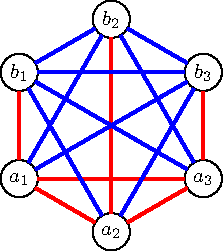
\includegraphics{figures/3_graph_3_cycle4}
\caption{Coloração de arestas do $K_6$ obtida durante demonstração.}
\label{graph:fig:cycle4}
\end{figure}
%%%%%%%%%%%%%%%%%%%%%%%%%%%%%%%%%%%%%%%%

Finalmente, a única configuração que nos resta é que cada $b_i$ pode ser identificado por uma aresta vermelha a um único $a_i$ e vice-versa. Sem perda de generalidade, podemos considerar que $c(b_1 a_1) = c(b_2 a_2) = c(b_3 a_3) = R$. Se alguma aresta $b_i b_j$ for vermelha, então $b_i b_j a_j a_i b_i$ forma um ciclo $C_4$ vermelho. Portanto, todas as arestas $b_i b_j$ são azuis, e temos a coloração dada na Figura~\ref{graph:fig:cycle4}, que possui um ciclo $C_4$ azul $b_2 b_1 a_2 b_3 b_2$. Portanto $r(C_4,C_4) \leq 6$.
\end{proof}
%%%%%%%%%%%%%%%%%%%%%%%%%%%%%%%%%%%%%%%%

O caso geral para ciclos foi completamente determinado, de forma independente, por Rosta~\cite{rosta1973ramsey} e Faudree e Schelp~\cite{faudree1974all}, e está caracterizado no Teorema~\ref{graph:thm:cycle} abaixo. Tendo em vista que estas demonstrações originais são bastantes envolvidas, uma simplificação recente foi desenvolvida por Károlyi e Rosta~\cite{karolyi2001generalized}.

%%%%%%%%%%%%%%%%%%%%%%%%%%%%%%%%%%%%%%%%
\begin{theorem}
\label{graph:thm:cycle}
Sejam $3 \leq m \leq n$ inteiros. Então,
\[r(C_m, C_n) = \begin{cases}
  6, & \text{se }m = n = 3 \text{ ou } 4;\\
  n + m/2 - 1, & \text{se }  n \text{ e } m \text{ pares}; \\
  \max\{n + m/2 - 1, 2n - 1\}, & \text{se } n \text{ ímpar e } m \text{ par};\\
  2n - 1 , & \text{se } m \text{ ímpar}.
\end{cases}\]
\end{theorem}
%%%%%%%%%%%%%%%%%%%%%%%%%%%%%%%%%%%%%%%%

Como $P_n$ é um subgrafo de $C_n$, temos que $r(P_m, P_n) \leq r(C_m, P_n) \leq r(C_m, C_n)$ para todo $n$ e $m$ inteiros. Como os números de Ramsey $r(P_m, P_n)$ estão determinados no Teorema~\ref{graph:thm:path} e o número $r(C_m, C_n)$, no Teorema~\ref{graph:thm:cycle}, obtemos, imediatamente, limitantes para $r(C_m, P_n)$. Resultados precisos, no entanto, foram obtidos por Faudree, Lawrence, Parsons e Schelp~\cite{faudree1974path}, e estão enunciados abaixo.

%%%%%%%%%%%%%%%%%%%%%%%%%%%%%%%%%%%%%%%%
\begin{theorem}
\label{graph:thm:pathcycle}
Sejam $m$ e $n$ inteiros. Então
\[r(C_m, P_n) = \begin{cases}
  2n - 1, & \text{se }3 \leq m \leq n, m \text{ ímpar};\\
  n + m/2 - 1, & \text{se }4 \leq m \leq n, m \text{ par}; \\
  \max\{m + \lfloor n/2 \rfloor - 1, 2n - 1\}, & \text{se } 2 \leq n \leq m, m \text{ ímpar};\\
  m + \lfloor n/2 \rfloor -1 , & \text{se } 2 \leq n \leq m, m \text{ par}.
\end{cases}\]
\end{theorem}
%%%%%%%%%%%%%%%%%%%%%%%%%%%%%%%%%%%%%%%%

Em particular, se $m$ e $n$ são pares e pelo menos um deles for maior que 4, então $r(P_m, P_n) = r(C_m, P_n) = r(C_m, C_n)$.

%%%%%%%%%%%%%%%%%%%%%%%%%%%%%%%%%%%%%%%%%%%%%%%%%%%%%%%%%%%%%%%%%%%%%%%%%%%%%%%%

\section{Árvores}

Seja $G$ um grafo simples. Dizemos que dois vértices $x$ e $y$ estão \indef{conectados} se existe um caminho em $G$ com uma extremidade em $x$ e outra em $y$. Note que esta relação é uma relação de equivalência no conjunto $V(G)$. Chamamos as classes de equivalência desta relação de \indef{componentes}. Dizemos que $G$ é \indef{conexo} se quaisquer dois vértices de $G$ estão conectados, ou seja, $G$ possui apenas uma componente.

%%%%%%%%%%%%%%%%%%%%%%%%%%%%%%%%%%%%%%%%
\begin{figure}[ht!]
\centering
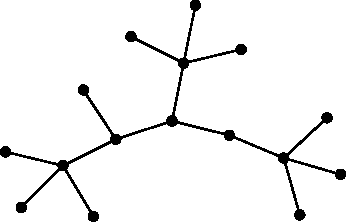
\includegraphics{figures/3_graph_4_tree}
\caption{Árvore com dezesseis vértices e dez folhas.}
\label{graph:fig:tree}
\end{figure}
%%%%%%%%%%%%%%%%%%%%%%%%%%%%%%%%%%%%%%%%

Um grafo que não possui ciclos como subgrafo é dito \indef{acíclico}.
Um grafo $G$ é chamado de \indef{árvore} se ele é conexo e acíclico. A Figura~\ref{graph:fig:tree} exemplifica uma árvore com dezesseis vértices. Árvores são grafos conexos minimais, isto é, a remoção de qualquer aresta de uma árvore a desconecta. Os grafos $P_n$ e $K_{1,n}$ são árvores.

Os vértices de uma árvore que possuem grau um são chamados de \indef{folhas}. A árvore da Figura~\ref{graph:fig:tree}, por exemplo, possui dez folhas. Pode ser mostrado que qualquer árvore com pelo menos dois vértices possui pelo menos duas folhas. A árvore $P_n$, por exemplo, possui exatamente duas folhas se $n \geq 2$.

Existem diversas maneiras equivalentes de se definir árvores. A seguir, listamos algumas propriedades de árvores que também podem ser tomadas como definições. De fato, se $G$ é um grafo simples com $n$ vértices, as seguintes proposições são equivalentes.

\begin{enumerate}[label=\arabic*.,itemindent=*]
  \item $G$ é uma árvore.
  \item $G$ é conexo e acíclico.
  \item $G$ é conexo minimal.
  \item $G$ é conexo e possui $n-1$ arestas.
  \item Todo par de vértices de $G$ está conectado por um único caminho.
\end{enumerate}

%%%%%%%%%%%%%%%%%%%%%%%%%%%%%%%%%%%%%%%%
\begin{figure}[ht!]
\centering
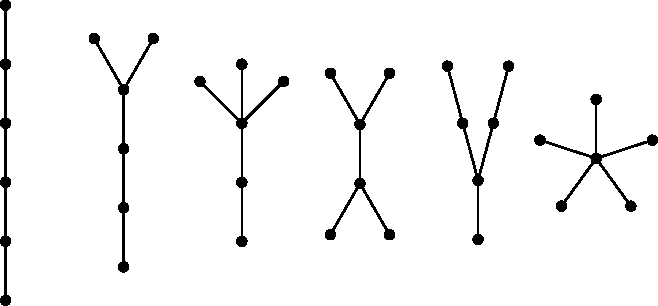
\includegraphics{figures/3_graph_5_tree6}
\caption{Todas as árvores com seis vértices.}
\label{graph:fig:tree6}
\end{figure}
%%%%%%%%%%%%%%%%%%%%%%%%%%%%%%%%%%%%%%%%

Para determinar números de Ramsey envolvendo árvores, precisamos de critérios para encontrar árvores como subgrafos de um grafo fixo. É de particular interesse que encontremos critérios não dependam da estrutura da árvore, mas apenas da quantidade de vértices. Nota-se pela Figura~\ref{graph:fig:tree6} que árvores com uma mesma quantidade de vértices podem ter estruturas radicalmente distintas. Mesmo assim, se $T$ é uma árvore de $n$ vértices, sempre encontramos $T$ como subgrafo de $K_n$, por exemplo. Podemos fazer ainda melhor com a seguinte proposição.

%%%%%%%%%%%%%%%%%%%%%%%%%%%%%%%%%%%%%%%%
\begin{proposition}
\label{graph:thm:treesub}
Seja $T$ uma árvore com $n$ vértices e $G$ um grafo com $\delta(G) \geq n-1$. Então $G$ possui uma cópia de $T$.
\end{proposition}
%%%%%%%%%%%%%%%%%%%%%%%%%%%%%%%%%%%%%%%%
\begin{proof}
Vamos provar por indução em $n$. Se $n = 2$, então $T \iso K_2$, logo o grafo $G$ possui uma cópia de $T$ se e somente se $G$ possui alguma aresta. Mas $\delta(G) \geq 1$, e assim, concluimos que $G$ possui uma aresta.

Considere agora que $n > 2$. Seja $G$ um grafo com $\delta(G) \geq n-1$. Seja $v \in V(T)$ uma folha. Como $d_T(v) =1$, existe apenas um vértice adjacente à $v$ em $T$; denote-o por $u \in V(T)$. Note que o grafo $T' = T - v$ também é uma árvore, uma vez que a remoção de uma folha não cria ciclos e não desconecta $T$. A árvore $T'$, no entanto, possui $n-1$ vértices. Por hipótese de indução, existe uma cópia de $T'$ em $G$. Seja $x \in V(G)$ o vértice que corresponde ao vértice $u \in V(T')$.
Por hipótese, temos que $d_G(x) \geq n-1$. Como existem apenas outros $n-2$ vértices em $T'$, isto implica que existe um vértice $y \in V(G)$ adjacente a $x$ que não foi utilizado na cópia de $T'$ em $G$. Unindo a cópia de $T'$ com a aresta $xy$, obtemos uma cópia de $T$ em $G$.
\end{proof}
%%%%%%%%%%%%%%%%%%%%%%%%%%%%%%%%%%%%%%%%

Com este resultado, podemos generalizar a Proposição~\ref{graph:thm:rpt} da seguinte maneira.

%%%%%%%%%%%%%%%%%%%%%%%%%%%%%%%%%%%%%%%%
\begin{proposition}
\label{graph:thm:ramseytree}
Seja $T$ uma árvore com $n$ vértices. Então
\[r(T,K_3) = 2n - 1.\]
\end{proposition}
%%%%%%%%%%%%%%%%%%%%%%%%%%%%%%%%%%%%%%%%
\begin{proof}
Note que o grafo $K_{n-1,n-1}$ não possiu triângulos e o seu complementar são duas cópias disjuntas de $K_{n-1}$, logo não possuem $T$ como subgrafo. Com isto, temos que $r(T,K_3) > 2n - 2$.

Seja $c$ uma $RB$-coloração de $G = K_{2n-1}$ que não possui $T$ vermelho ou $K_3$ azul. Pela Proposição~\ref{graph:thm:treesub}, se $\delta(G_R) \geq n-1$, então $c$ possui $T$ vermelho, logo, existe um vértice $v$ com $d_R(v) \leq n - 2$. Portanto $d_B(v) \geq n$. Se existir alguma aresta azul com ambas as extremidades em $N_B(v)$, unindo-as com $v$ forma-se um $K_3$ azul.
Portanto $N_B(v)$ só possui arestas vermelhas. Como $|N_B(v)| \geq n$, $c$ possui um $K_n$ vermelho. Em particular, $c$ possui uma cópia de $T$ vermelha, contradizendo nossa hipótese. Concluímos então que $r(T,K_3) \leq 2n - 1$.
\end{proof}
%%%%%%%%%%%%%%%%%%%%%%%%%%%%%%%%%%%%%%%%

Finalmente, podemos obter os números de Ramsey de árvores contra grafos completos de qualquer ordem.

%%%%%%%%%%%%%%%%%%%%%%%%%%%%%%%%%%%%%%%%
\begin{theorem}[Chvátal~\cite{chvatal1977tree}]
\label{graph:thm:chvatal}
Seja $T$ uma árvore com $n$ vértices. Então
\[r(T,K_s) = (s-1)(n-1) + 1.\]
\end{theorem}
%%%%%%%%%%%%%%%%%%%%%%%%%%%%%%%%%%%%%%%%
\begin{proof}
Observe que o grafo de Turán $T_{s-1}(n-1)$ não possui $K_s$ como subgrafo. Além disso, o seu complementar consiste de $s-1$ cópias disjuntas de $K_{n-1}$, que não possuem $T$ como subgrafo. Isto nos dá que $r(T,K_s) > v(T_{s-1}(n-1)) = (s-1)(t-1)$.

Para o limitante superior, vamos proceder por indução em $s$. O caso $s = 3$ está demonstrado na Proposição~\ref{graph:thm:ramseytree}. Agora, suponha que $c$ seja uma $RB$-coloração de $G = K_{(s-1)(n-1) + 1}$ sem $T$ vermelho e sem $K_s$ azul.
Pela Proposição~\ref{graph:thm:treesub}, se $\delta(G_R) \geq n-1$, então $c$ possui $T$ vermelho, logo, existe um vértice $v$ com $d_R(v) \leq n - 2$. Portanto $d_B(v) \geq (s-1)(n-1) - n + 2 = (s-2)(n-1) + 1$.
Como $N_B(v)$ possui pelo menos $(s-2)(n-1) + 1$ vértices, pela hipótese de indução, $N_B(v)$ possui um $T$ vermelho ou um $K_{s-1}$ azul. Mas como $c$ não possui $T$ vermelho, $N_B(v)$ possui um $K_{s-1}$ azul. No entanto, unindo o vértice $v$ à cópia azul de $K_{s-1}$, obtemos um $K_s$ azul, o que é absurdo. Portanto, $r(T,K_s) \geq (s-1)(n-1) + 1$.
\end{proof}
%%%%%%%%%%%%%%%%%%%%%%%%%%%%%%%%%%%%%%%%

Tendo em vista este teorema e outros resultados similares, Burr e Erdös~\cite{burr1983generalizations} conjecturaram em 1983 que
\[ r(H,K_s) = (s-1)(v(H) - 1) + 1\]
para todo $s$ fixo e $H$ suficientemente esparso. Um grafo pode ser considerado esparso de diversas maneiras diferentes. De fato, pelo mesmo argumento utilizado acima no Teorema de Chvátal, se $H$ é um grafo conexo, então $r(H,K_s) \geq (s-1)(v(H) - 1) + 1$ . Um grafo $H$ para o qual vale a igualdade é dito $s$-bom.
Burr e Erdös conjecturaram que se $H$ é uma família de grafos com grau médio limitado, então $H$ é $s$-bom.

Esta conjectura foi desprovada por Brandt~\cite{brandty1996expanding}, mas resultados similares valem para grafos esparsos em outros sentidos. Por exemplo, Burr e Erdös mostraram que se $H$ possui largura de banda\footnote{A largura de banda de um grafo $G$ é o menor inteiro positivo $l$ tal que existe uma ordenação $v_1, \dots, v_n$ dos vértices de $G$ de forma que toda aresta $v_i v_j$ satisfaz $|i - j| \leq l$.} limitada, então $H$ é $s$-bom. Este resultado foi estendido por Allen, Brightwell e Skokan~\cite{allen2013ramsey} para grafos com largura de banda até $o(\log n / \log \log n)$ e grafos com grau médio limitado e largura de banda $o(n)$.

Outros resultados foram obtidos para famílias específicas. Por exemplo, Pontiveiros, Griffiths, Morris, Saxton e Skokan~\cite{pontiveros2014ramsey} estudaram o caso do hipercubo $Q_n$, isto é, o grafo com conjunto de vértices $\{ 0, 1 \}^n$ e arestas entre pares de vértices que diferem em exatamente uma coordenada. O hipercubo possui $N=2^n$ vértices, grau médio $\log_2(N)$ e largura de banda aproximadamante $N/\sqrt{\log N}$, e portanto, não está coberto pelos resultados mais genéricos menciodados.
Foi mostrado em~\cite{pontiveros2014ramsey} que $r(Q_n, K_s) = (s-1)(2^n -1) + 1$ para $n$ suficientemente grande.


%%%%%%%%%%%%%%%%%%%%%%%%%%%%%%%%%%%%%%%%%%%%%%%%%%%%%%%%%%%%%%%%%%%%%%%%%%%%%%%%


%%%%%%%%%%%%%%%%%%%%%%%%%%%%%%%%%%%%%%%%%%%%%%%%%%%%%%%%%%%%%%%%%%%%%%%%%%%%%%%%
